\documentclass[a4paper,twoside]{revtex4-1}
\usepackage[font=small,format=plain,labelfont=bf,up,textfont=it,up]{caption}
\usepackage[margin=2.5cm]{geometry} % change margin
\usepackage{subfigure}  %subfigures
\usepackage{graphicx}	%include graphics
\usepackage{fullpage}	
\usepackage{courier}     %\ttfamily
\usepackage{amsmath}	%Mathematics
\usepackage{mathtools} % "amsmath++"
\usepackage{amssymb}	%the R of real number, C of complex, etc.
\usepackage{float}		%To place figures where I want them
\usepackage{braket}		%The Quantum Mechanical Dirac notation: | > , < | , < > 
\usepackage{parskip}		
\usepackage[dvipsnames]{xcolor}		 %colored text
\usepackage{sidecap}		%Figure with a caption on the side
\usepackage{chngcntr}         %To adjust numbering of sections without having to use Chapters
\usepackage{nicefrac}


% Symbols used in model:
% Rate's (allways comes in handy)
\newcommand{\rate }[1]{\ensuremath{k_{\text{#1}}} }

%% Parameters: MFPT 
\newcommand{\lambdaS}{\ensuremath{\lambda_{\text{S}}  }}
\newcommand{\lambdaL}{\ensuremath{\lambda_{\text{L}}  }}
\newcommand{\gap}{\ensuremath{\delta_{\text{gap}}  }}

\newcommand{\weigthS}{\ensuremath{w_{\text{S}}}}
\newcommand{\LDNA}{\ensuremath{L_{\text{DNA}} }}


\newcommand{\Precap}{\ensuremath{P_{\text{RC}}}}
\newcommand{\Pub}{\ensuremath{P_{\text{ub}}}}
\newcommand{\PS}{\ensuremath{P_{\text{S}} }}
\newcommand{\PR}{\ensuremath{P_{\text{R}} }}
\newcommand{\ProbS}{\ensuremath{\rho_{\text{S}} }}
\newcommand{\ProbR}{\ensuremath{\rho_{\text{R}} }}
\newcommand{\NumberReturns}{\ensuremath{\overline{n}_{\text{return}}}}

%% Parameters: MonteCarlo simulation 
\newcommand{\Rmax}{\ensuremath{R_{\text{max}} }}
\newcommand{\Rprot}{\ensuremath{R_{\text{protein}} }}
\newcommand{\lambdaexcl}{\ensuremath{\lambda_\text{excl}} }


%% for the captions of the Supplemental Figures:
\newcommand{\figA}{\ensuremath{\textbf{(A)}}}
\newcommand{\figB}{\ensuremath{\textbf{(B)}}}
\newcommand{\figC}{\ensuremath{\textbf{(C)}}}
\newcommand{\figD}{\ensuremath{\textbf{(D)}}}

%% change style of section numbering
\renewcommand{\thesection}{\Alph{section}}
\renewcommand{\thesubsection}{\Roman{subsection}}

%% change the style of equation numbering 
\renewcommand{\theequation}{\arabic{equation}} 
%% suppress page numbering 
\pagenumbering{gobble}


\newcommand{\shuttletime}{\ensuremath{\Delta t_{\rm{shuttle}}}}
\newcommand{\tauBC}{\ensuremath{\Delta \tau_{\rm{BC}}}}
\newcommand{\tauCB}{\ensuremath{\Delta \tau_{\rm{CB}}}}


\newcommand{\singletargetdist}{\ensuremath{p_{\rm{bound}}}}
\newcommand{\shuttledist}{\ensuremath{P_{\rm{shuttle}}}}
\newcommand{\xPolT}{\ensuremath{x_{\rm{poly-T}}}}
\newcommand{\xTarget}{\ensuremath{x_{\rm{Target}}}}
\begin{document}
\begin{center}
{\bf \Large {Brief summary modeling}}
\vspace{10pt} \\ 
Misha Klein \quad Behrouz Eslami \quad Martin Depken  \\  
\end{center}




\section*{The free-energy landscape}
We build a physical model of Cas-gRNA binding to its DNA substrate. The guide-loaded protein can either be unbound - being in solution - bound to the PAM or having formed an R-loop (intermediate) of a length between 1 and the guide-length (20nt for Cas9) (see figure \ref{dCas9_model}). Furthermore we envision a 'zipper-like' process in which the R-loop grows/shrinks with single nulceotide increments/decrements. The model is therefore fully described by the set of 21 forward rates and backward rates. These rates could in principle depend on both the length of the hybrid formed, termed 'position dependence', as well as sequence content. However, for now we attempt to find overarching targeting behaviour, which should be sequence independence. With this in mind, we assume there are just 3 distinct forward rates: a binding rate from solution to PAM, an internal forward rate while extending the R-loop and a rate from the PAM bound state to initiate the R-loop. The latter is to a good part insired by the bulk data shown by your group implying that initiation the R-loop is the rate limmiting process for cleavage. 
\\ \\ 
To obtain the backward rates, we chose to model the free-energy of every intermediate state and use the detailed balance condition to relate those - via the forward rates just mentioned - to the desired backward rates.
\begin{equation}
	\rate{b}(i) = e^{+\epsilon(i)} \times \rate{f}(i-i)
\end{equation}
with:
\begin{equation}
	\epsilon(i) = \begin{cases}
	\epsilon_{PAM} & \text{at PAM} \\
	-\epsilon_C(i) & \text{for a match} \\
	\epsilon_I(i) - \epsilon_C(i)  & \text{for a mismatch}
	\end{cases}  
\end{equation}
Given a set of energy differences that make up the  free energy landscape (see figure \ref{free_energy_cartoon}) and the three remaining forward rates, we can set up the appropriate evolution equation for the set of populations in each of the states of our model:
\begin{equation}
	\frac{\mathrm{d} \vec{P}(t)}{\mathrm{d}t} = M \vec{P}(t)
\end{equation}
Solving this set of Master equations essentially gives us access to any observable quantity of the system. 

\begin{figure}[H]
	\centering
	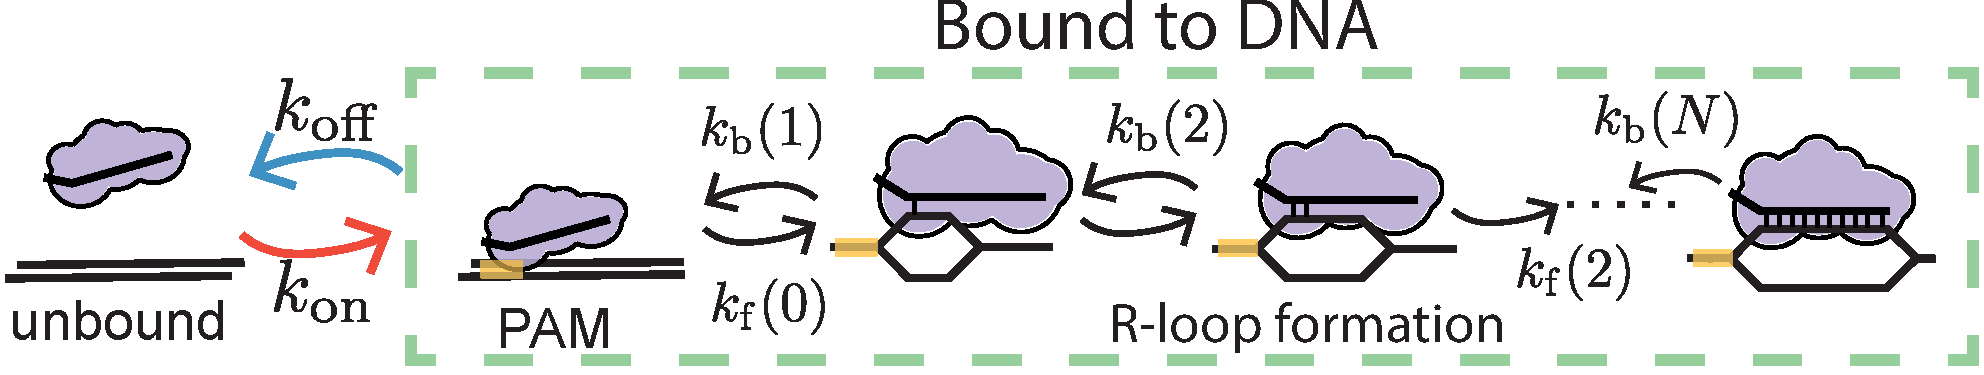
\includegraphics[width=\textwidth]{dCas9_modelling}
	\caption{Kinetic model of dCas9 (un)binding dynamics. On the microscopic level, we treat every configuration with a single basepair added/removed to the R-loop as a (meta-)statble intermediate.  On the more coarse-grained level, all states in which any kind of R-loop is formed, or the protein is attached at the PAM site, are considered to contribute to the population of bound molecules ($P{\rm{bound}}(t) = \sum_{n='PAM'}^{N} P_i(t)$). }
	\label{dCas9_model}
\end{figure}


\begin{figure}[H]
	\centering
	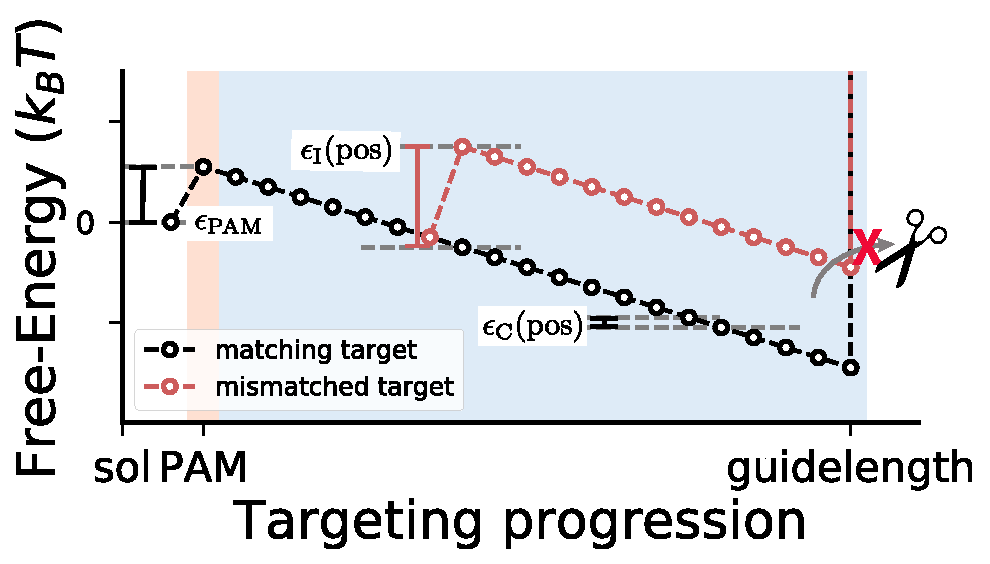
\includegraphics[scale=0.75]{cartoon_energy_landscape_edit}
	\caption{microscopic free-energy landscape for the active enzyme. Parameters are 20 gains/penalties for matches $\epsilon_C$, 1 energy of the PAM bound state $\epsilon_{PAM}$, 20 mismatches penalties $\epsilon_I$ and 3 distinct-valued forward rates (binding rate from solution to PAM, the rate from PAM to enter the R-loop and the rate of adding a basepair to the R-loop).  }
	\label{free_energy_cartoon}
\end{figure}




\section*{Training using data Boyle et al.}



\begin{figure}[H]
	\centering
	\includegraphics[width=\textwidth]{frame_800}
	\caption{Costum build simulated annealing algorithm to fit our model to experimental data. Shown are: (top left) On-target free-energy landscape, (top right) mismatch penalties, (bottom right) comparison to single missmatch data and (bottom left) comparisson to all double missmatch data.  }
\end{figure}


\begin{figure}[H]
	\centering
	\includegraphics[scale=0.75]{all_fits_to_Boyle}
	\caption{On-target free-energy landscape after 66 repititions of the SA-algorithm. By overlaying the results from multiple fits - that are all equally good in performance ($<5\%$ difference in predicted associated rates)- we see what features are very strongly determined by the data and which are not so much. }
\end{figure}


\begin{figure}[H]
	\centering
	\includegraphics[scale=0.5]{correlation_plot_Boyle}
	\caption{Correlation between training data and model prediction: 0.94367427}
\end{figure}





\section*{Testing using data Finkelstein lab}
After having characterised the model parameters using the data from Boyle et al. we can without the use of any free-parameters predict the outcome of your experiment. 

\begin{figure}[H]
	\centering
	\includegraphics[width=\textwidth]{ABA_Hill_Eqn}
	\caption{We mimic the procedure described in Jung et al. by solving the master equation for the bound fraction after 10 minutes for different concetrations. Just as described, we obtain the ABA by fitting the Hill Eqn to the obtained datapoints to get the dissociation constant and taking its logarithm.  }
\end{figure}

\begin{figure}[H]
	\centering
	\includegraphics[width=\textwidth]{correlation_plot_Ilya}
	\caption{Model prediction versus your data. }
\end{figure}

\begin{figure}[H]
	\centering
	\includegraphics[width=\textwidth]{double_mm_heatmap}
	\caption{all double mismatches }
\end{figure}



\begin{figure}[H]
	\centering
	\includegraphics[width=\textwidth]{block_mm_experiment}
	\caption{data for all sets of consequetive mismatches  }
\end{figure}

\begin{figure}[H]
	\centering
	\includegraphics[width=\textwidth]{block_mm_prediction}
	\caption{prediction of $\Delta$ABA for consequetive mismatches  }
\end{figure}


\begin{figure}[H]
	\centering
	\includegraphics[width=\textwidth]{blocks_collapse_first_position}
	\caption{Data and prediction for consequetive mismatches after averaging over the block length. }
\end{figure}

\begin{figure}[H]
	\centering
	\includegraphics[width=\textwidth]{single_mm}
	\caption{data and prediction of $\Delta$ABA for single mismatches.  }
\end{figure}




\newpage 
\section*{Translating to active Cas9}
Translating between Cas and (d)Cas: 
\begin{figure}[H]
	\centering
	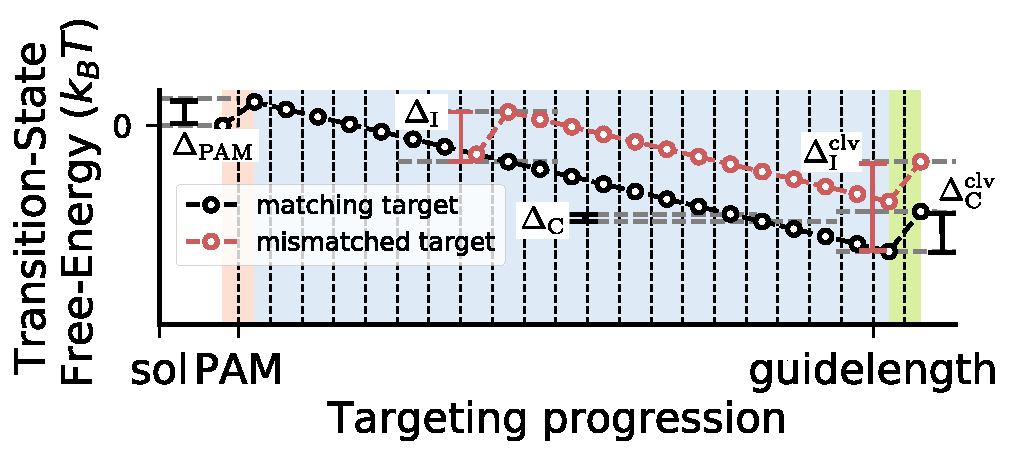
\includegraphics[width=\textwidth]{cartoon_transition_state_landscape_v2_edit}
	\caption{microscopic free-energy landscape for the active enzyme. Parameters are 20 gains/penalties for matches $\epsilon_C$, 1 energy of the PAM bound state $\epsilon_{PAM}$, 20 mismatches penalties $\epsilon_I$ and 3 distinct-valued forward rates (binding rate from solution to PAM, the rate from PAM to enter the R-loop and the rate of adding a basepair to the R-loop). Given this is the landscape for the active enzyme, there is another rate in play: the intrisic rate to cleave (or the associated forward barrier). }
\end{figure}

\end{document}

